\documentclass{article}
\usepackage[utf8]{inputenc}
\usepackage{graphicx}
\usepackage[hidelinks]{hyperref}
\usepackage{listings}
\usepackage{xcolor}


\definecolor{codegreen}{rgb}{0,0.6,0}
\definecolor{codegray}{rgb}{0.5,0.5,0.5}
\definecolor{codepurple}{rgb}{0.58,0,0.82}
\definecolor{backcolour}{rgb}{0.95,0.95,0.92}

\lstdefinestyle{codestyle}{
    backgroundcolor=\color{backcolour},   
    commentstyle=\color{codegreen},
    keywordstyle=\color{magenta},
    numberstyle=\tiny\color{codegray},
    stringstyle=\color{codepurple},
    breaklines=true,
    numbers=left,
}

\lstset{style=codestyle}

% TODO: Add better titles for methodology
% TODO: Summary of Methodology -> Give Some insights as to what I did.
% TODO: Tone Down Ethical Considerations -> Maybe some contributions here ??
% TODO: Twitter case Study -> 

\pagestyle{headings}
\begin{document}
\begin{titlepage}
\title{TRACKING MALICIOUS TRANSACTIONS IN CRYPTOCURRENCIES}
\author{Bhavish Dhanda {\\ Supervisor: Dr Hassan Asghar} {\\ Co-Supervisor: Dr Benjamin Zhao}}
\date{}
\end{titlepage}
\maketitle
\begin{center}
    
\includegraphics[width=0.7\linewidth]{logo.jpg}\\[4ex]
    Department of Computing and Engineering\\
    Macquarie University\\
    Australia
\end{center}
\pagebreak

\begin{center}
    \section*{ACKNOWLEDGEMENTS}
        I would like to acknowledge and give my warmest thanks to my supervisor Dr Hassan Asghar and co-supervisor Dr Benjamin Zhao who made this work possible. Their guidance and advice carried me through all the stages of writing my project. 
        \pagebreak
    \section*{STATEMENT OF CANDIDATE}
        I hereby declare that the work, which is being presented in the Thesis, entitled “Tracking malicious transaction in Cryptocurrencies”, in partial fulfillment of the requirement for the award of the degree of Bachelor of Software Engineering (Honours) in the department of Engineering, Macquarie University.  This thesis is an original piece of research work under the guidance of Dr Hassan Asghar and Dr Benjamin Zhao. The matter embodied in this thesis has not been submitted for the award of any other degree of any other academic institution.
        \pagebreak

\tableofcontents
\pagebreak
\listoffigures
\pagebreak
\lstlistoflistings
\pagebreak

\section*{Abstract}
    Cryptocurrencies form what is called the new decentralized finance world of digital finances. They have become increasingly popular in the recent few years and with this technology becoming more and more accessible, the number of users of this form of payments have grown exponentially.On of the other side of coin, this mass usage of this technology gives a small percentage of people of hide in plain sight and do illegal activities. These people who are involved in such malicious activites are also supported by the anonymity features of this form of payments. 

\end{center}

\pagebreak

\section{Introduction}
    Cryptocurrencies have become the modern form of decentralized finance giving the general public a level of visibility and control over financial systems that we could never imagine while using traditional financial systems. Their adoption has increased exponentially in the last few years with a few countries even deciding to make it a legal tender for their day to day transactions. Such countries include but are not limited to Central African Republic, El Salvador \cite{browne_2022} where Bitcoin has been deemed as a legal form of tender by the local authorities. 

    The striking difference between so-called decentralized finance\cite{zetzsche_arner_buckley_2020} formed by cryptocurrencies and traditional banking systems the type of ledger they maintain, and how the currency is controlled. Decentralized as the word suggests means that the control is not the in hands of a single person or entity rather the entire network, in this case, all the people using and servicing the cryptocurrency influence all the decisions that are made which include, the price largely controlled by supply and demand and the number of people mining and other factors, validation of transactions is normally done by validation nodes inside the networks and similar functions all are done by the public nodes inside the network. The second major factor that contributes to this decentralization is the public ledger these currencies maintain in contrast to a centralized secured ledger maintained by traditional banking systems where only certain authorized users can access the ledger, in the case of cryptocurrencies, anyone can access the ledger and see all sorts of information stored in a typical currency ledger which includes account balances, transactions made etc. 

    Now with this increased popularity there is a growing problem of illegal use of cryptocurrencies both through the dark web markets and also through direct P2P transactions. Sesha Kethineni1 and Ying Cao1 \cite{kethineni_cao_2019} have done a very good job to highlight the seriousness of the problem we are trying to tackle. They explain how modern cryptocurrencies such as Monero\cite{getmonero.org}, Dash\cite{dash_2022} and a few others who are built upon existing currencies with the sole purpose of improving privacy are being more and more used for illegal activities. Along with that they explain how some countries as planning to introduce cryptocurrencies as their mainstream form of payment. As much as it seems like this move this move is disliked by the more powerful countries like US, smaller countries see it as a way of achieving financial freedom US's payment systems. But this increasing accessibility gives people who are involved in illegal activities the perfect opportunity to hide in plain sight. 


    \textbf{Our goal in this paper is to find ways to track down on these malicious transactions and to try and get as close as possible to the real world entity behind these activities.}

    In the following sections we will go through everything mentioned above in detail starting with background about cryptocurrencies and the problem itself, followed by reviewing some work already done by researchers in this field to understand what can we learn from their work, and then we will discuss some ethical considerations made and why were they made in this piece of work. In the last few sections we will go through our methodology and the reasoning behind including some decisions made and why we made them, after which we will do some critical analysis of this work, followed by some ideas of potential future work people can undertake taking into account lessons learnt from our research and concluding with a \textbf{short and brief} conclusion about the paper.

\pagebreak

\section{Background}
    
    \subsection{What are cryptocurrencies}

        Cryptocurrencies are a modern form of digital decentralized currencies which aim to put all the control of a currency and how it works in the hands of the consumers. The distinguishing factor between the conventional currencies we normally use and crypto is first its operation of a public ledger and second decentralized control. Now, every currency needs to maintain a ledger to keep track of the consumers, their activites i.e. the transactions, their account balances, in traditional banking systems all of this information is confidential and only a select group of people have access to it whereas in the cryptocurrencies everything is public, anyone can download the blockchain on their systems or access it through a number of APIs available these days to look at this information. However with all this information, it doesn't mean that you know how much money someone has because cryptocurrencies hide their users' identity behind wallet addresses and there is no direct link between the real work identity of a person and his wallet address. So you can check how money there is in a wallet address, the transactions the address has made but cannot check who operates/owns the wallet address.


    \begin{figure}
            \centering
            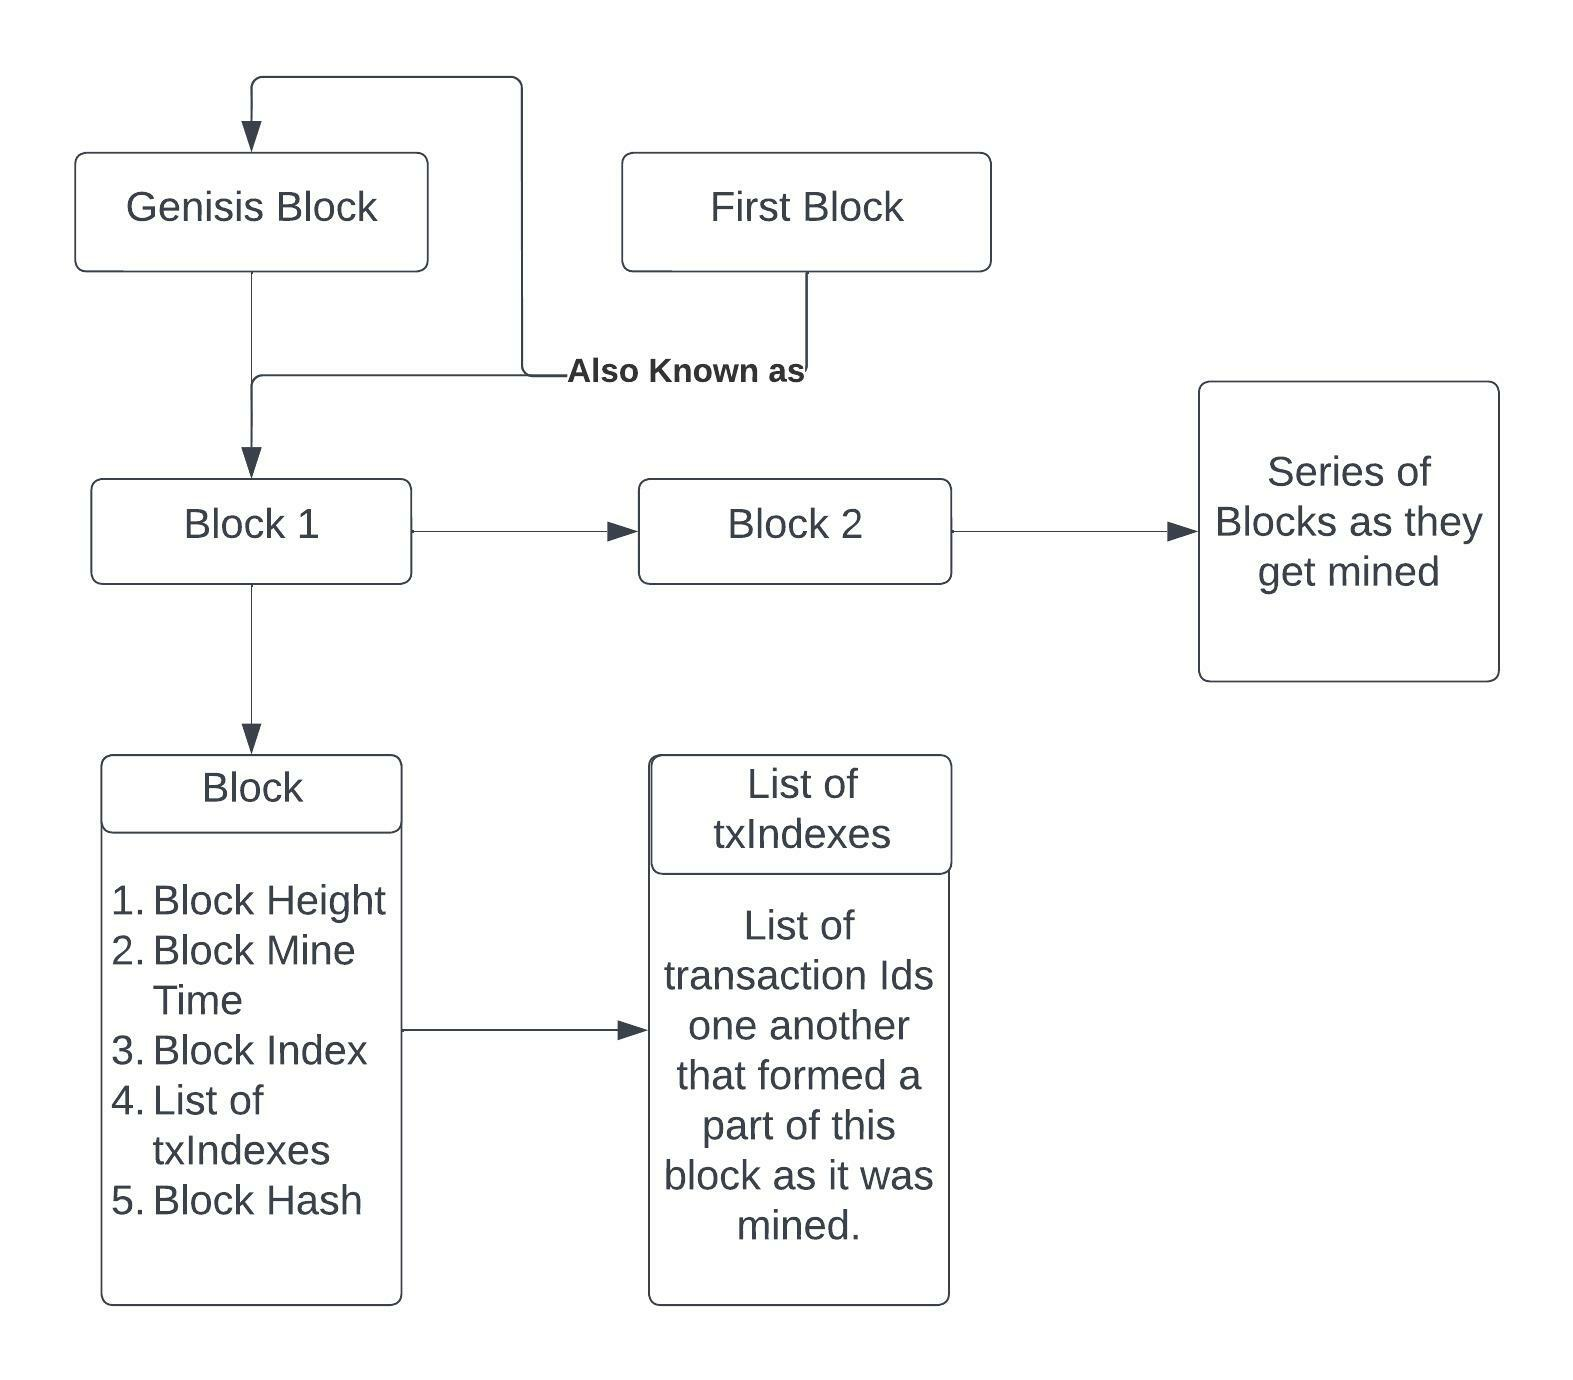
\includegraphics[width=150mm,scale=0.7]{Simple Blockchain.jpeg}
            \caption{A simple Blockchain Data Structure}
            \label{Figure 3}
        \end{figure}
        
\pagebreak

    \subsection{How do cryptocurrencies work?}
    
    
        Before we actually start exploring our area of research we need to be aware of how cryptocurrencies technically operate. To simplify things we will be using Bitcoin as our reference to explain the technical architecture.

        As said earlier all currencies need a ledger to work so in case of cryptocurrencies it is the blockchain itself. Blockchain could be any is essentially is a Linked List \cite{} of Blocks put one after another. Each Block inside the blockchain is a primarily a collection of transaction with some other metadata associated. Modern cryptocurrencies work on maintaining a public ledger which is the distinguishing factor of these currencies with the standard paper currencies that we have been using for ages. 

        In terms of actual decentralized operation of the currency, it works on the concept of a P2P network, that means in order to make a transaction on the currency you can connect directly to the other party without the oversight/involvement of a third party in the middle. Apart from that a large number of nodes/clients join the P2P network to host the currency and perform additional tasks such as mining, validation in return for some reward which depends on the currency itself. This is how the decentralization is enable the transactions are not managed or approved by a single entity or person rather a network of nodes on the P2P network known as validator nodes, same goes for miners, there are nodes on the network that perform mining and they are interacting directly with the blockchain so this eliminates the need to having to keep control of the currency in the hands of a single person or an entity.

\pagebreak

    \subsection{How do cryptocurrencies preserve privacy}

        Cryptocurrencies work on the concept of wallet addresses which is similar to having a bank account at any traditional financial institutions. Wallet account is the bank account number you get when opening up a bank account for the first time. That means any future transactions, enquiroes, would be using that account number as a reference. In the same way cryptocurrencies use the wallet address for any transcations, also as your identity on the currency network and ledger to store information. 

        The point at which the difference arrises between a traditional financial instituion like a bank and a cryptocurrency is where the account number / wallet address is generated. Normally a bank is requred to perform know you customer also known as KYC steps before they can issue an account number to validate the person's identity who is opening the bank account but in cryptocurrencies there is no such validation. A user can just create his own wallet address by providing no informaiton at all and this way he can issue as many wallet addresses for himself or anyone, in fact users of cryptocurrencues are actually encouraged to create a new wallet address for every transaction they perform on the blockchain to maximise their privacy. 
        
        This way when a customer has wallet address all his interactions to and within the blockchain would be through the address which has no information at all linked to his real world personal identity. He can do whatever he wants on the blockchain but all that would be left in the end is the wallet address which in no way shape or form would have enough information to even closely link to his real identity. But in contrast if this link is revealed by any way possible such as leaking of this information, the customer is completely exposed meaning, everyone can see how much money the user holds, how many transactions were made and with whom and everything linked to his wallet address. This way cryptocurrenciues are known to be pseudo-anonymous as they are normally and ideally extermaly anonymous but in case of leakage of information will preserve no privacy at all.

\pagebreak

    \subsection{Mixers}
        
        \begin{figure}[!htb]
            \centering
            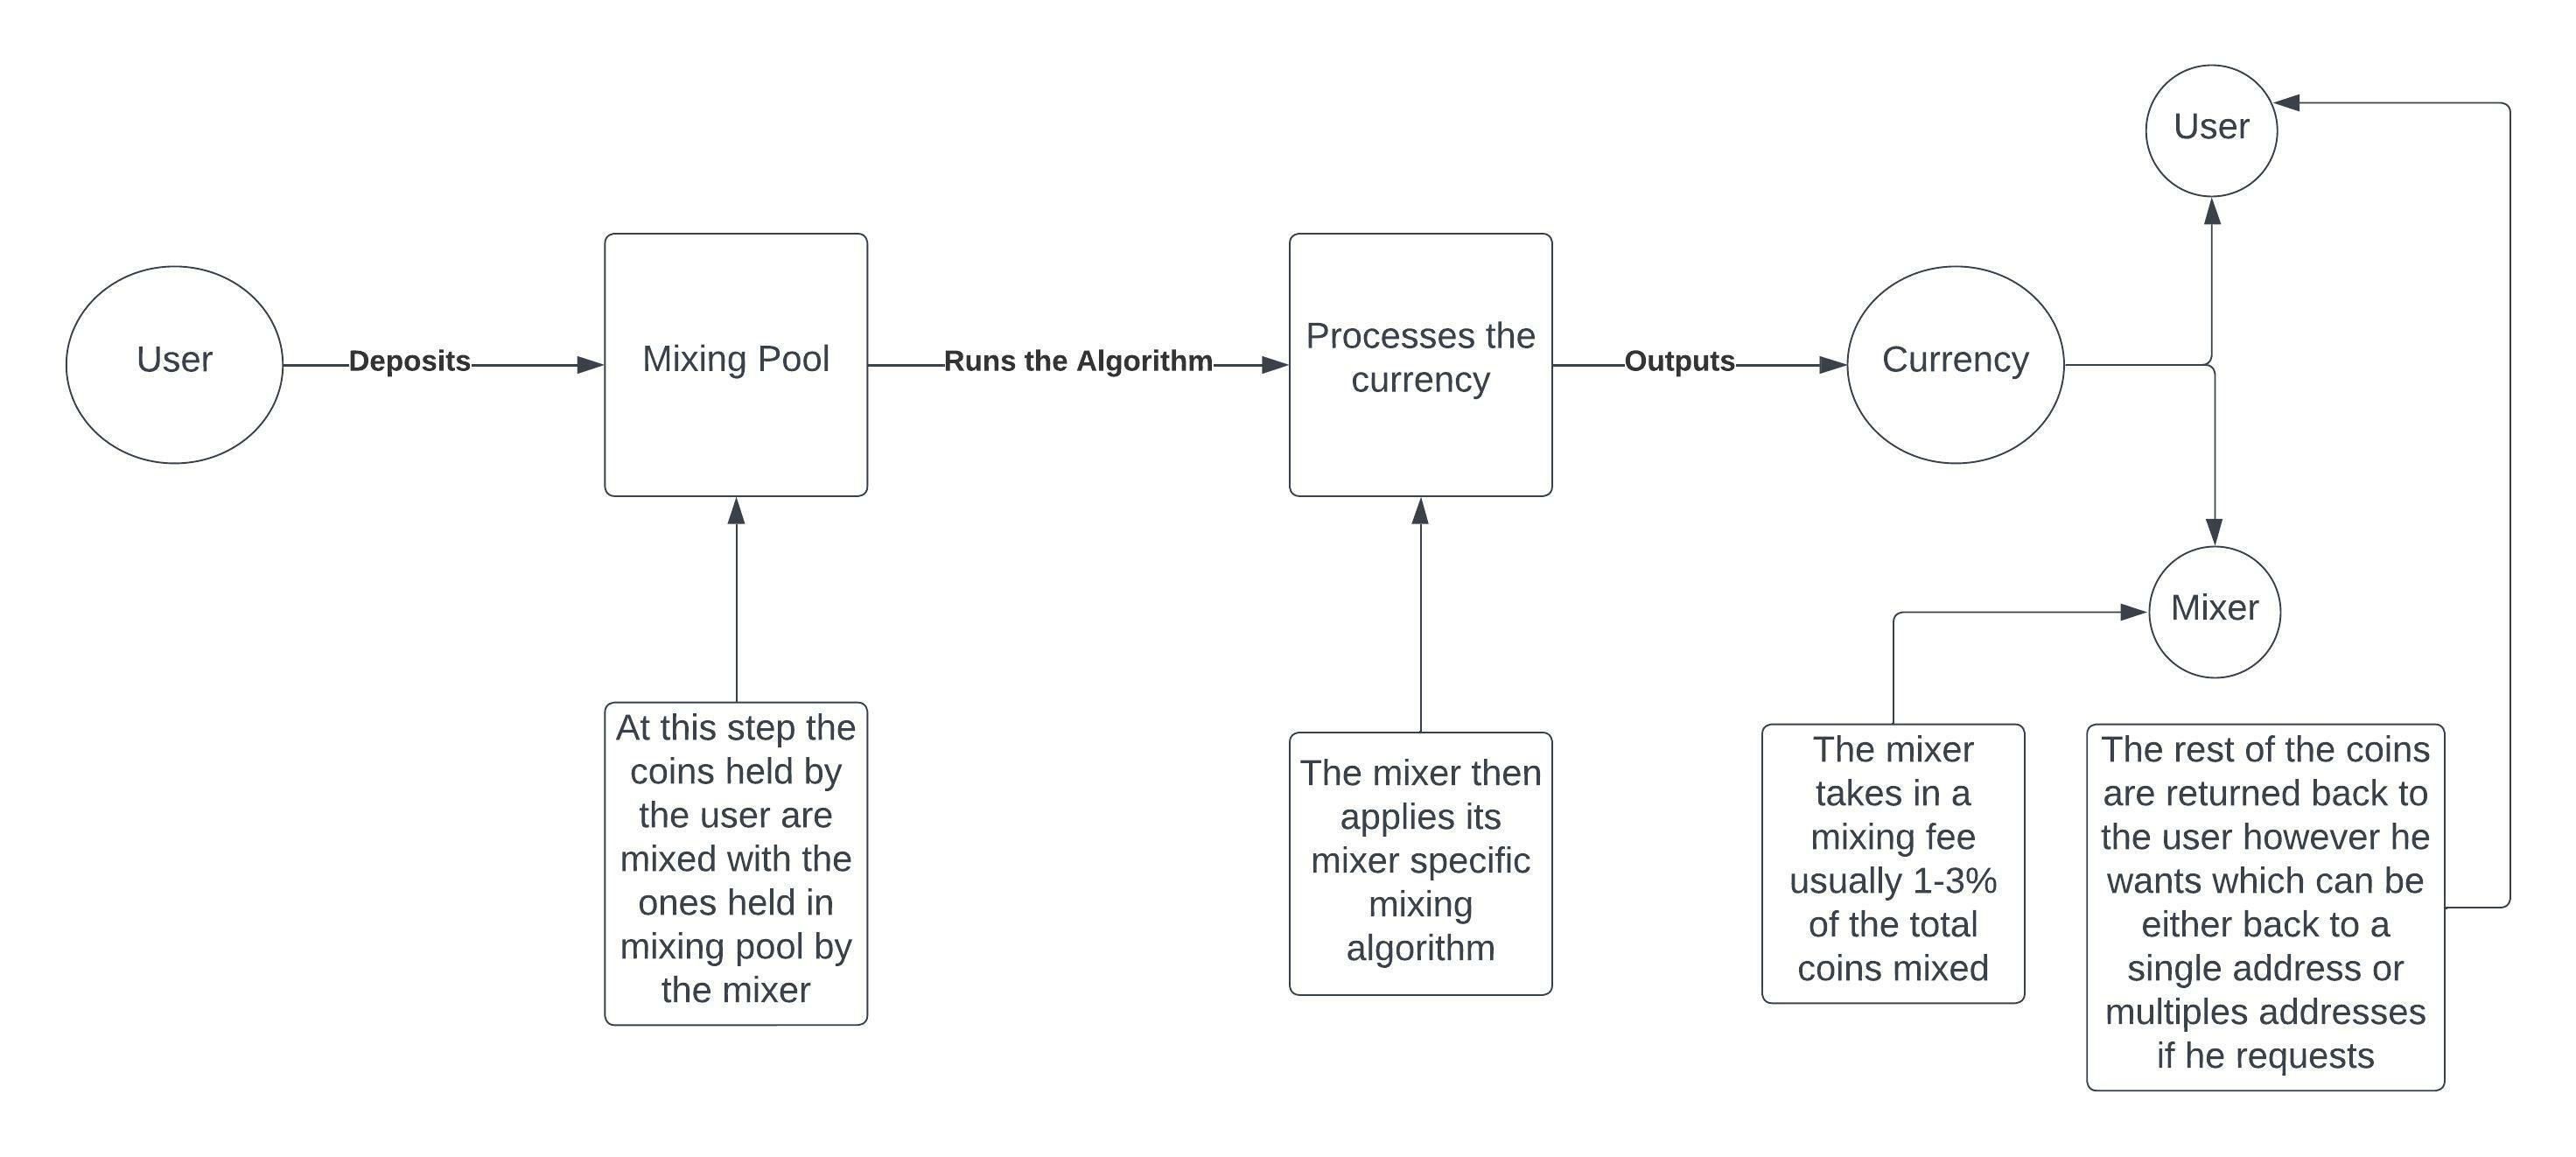
\includegraphics[width=150mm,scale=0.7]{Mixers.jpeg}
            \caption{Working of a basic mixing service}
            \label{Figure 3}
        \end{figure}
        
        Now that we are across how cryptocurrencies work, it is important we discuss about mixers as well as they introduce another dimension of complexity in the problem we are trying to solve.
        
        Mixers were developed with the sole purpose to improve the privacy of users using the blockchain and reduce traceability of transactions. Mixers as the word suggest perform mixing, what they mix is the addresses with others so that there is no direct link between the source and target address thereby giving the appearance that the money in the target address came from the address generated by the mixing service. We also need to keep in mind that by using mixers the traceability of the source to the target decreases but is never eliminated so these can in fact when searched extensively can be broken through to some extent, we will cover an example of such work in the related works section about mixers below.
        
         The way mixers work as highlited in fig \ref{Figure 3} is
        \begin{enumerate}
            \item The user transfers his currency to be mixed from his wallet to the mixing service's wallet. At this point all the user has is a withdrawal note from the mixer which indicates that the user holds funds in the mixing pool. Now this note can differ from case to case on how the user requested the funds to the be dispatched. For instance some users do not want their funds to be released immediately so that hold on to that note until they want them back, some want their funds to be sent to a different address and some mixing services also give the option to send money to multiple output address so that is what the withdrawal note states.
            \item After the money is deposited in the mixing pool, it becomes a part of the mixing pool with no direct association to the person who deposited the money. Now at this stage the mixing pool applies it mixing algorithm which is usually unique to the pool itself with the end goal of reducing traceability. 
            \item Now that the mixer has done his job the output currency from the mixing algorithm is supposed to be sent back to the user. This is the point where the mixer deducts its fee which is usually 1 - 3 percent and sends back the rest of the amount to the user wherever he requested them.
        \end{enumerate} 

\pagebreak

    \subsection{Dark Web Markets}
    
        To understand the role of cryptocurrencies in malicious activity it is important we understand what dark web markets are, and how they work to preserve the privacy of its users. Dark markets are essentially online shopping platforms like Amazon, Alibaba, etc but are used and developed for illegal activities like buying and selling illegal goods and services. Dark Web Markets are extremely popular amongst people trying to hide their online presence because they can only be accessed behind a hidden network and a private browser which ensures there is no leakage of information. These are usually access through The Onion Router also known as TOR\cite{tor_project_|_anonymity_online} which is basically an open source software for enabling anonymous communication. The malicious activity on these networks has only increased after the launch of cryptocurrencies, as most of them have now started to accept cryptocurrencies, breaking further the single point where there could be traceability. Normal online transactions can be traced by the financial institutions where the account belongs, one can be caught performing cash transaction but introducing cryptocurrencies breaks this final link as well.
    
        These are an extremely old type of illegal markets which have managed to remain in circulation even after various blow-backs from the authorities by having a successor every time one is taken down. Silk Road\cite{Silk_Road} was one such example which was one of first marketplace of such kind, which was founded in 2011 by a group of group of people, to only a select group of people and later expanded into the wider audience. As silk road was opened to the wider audience its number of users and the income increase as well along with sparking an interest of the authorities towards this. Eventually in 2013, this was shut down by the authorities but the concerning fact was that this did not give a lesson to the people to stop these services instead this lead and inspired to people working to launch Silk Road 2.0 shortly after. Another example of such service which came in the highlights was AlphaBay which was founded by Christin who was the one of the people who originally launched Silk Road. As highlited by Hiramoto Et al\cite{hiramoto2020measuring} in their research that AlphaBay was the second biggest dark web market during the period it was active based on its total revenue. And out of this revenue it was estimated that there were around 450 millions worth of 4 million transactions just in Bitcoin and introduction of mixing services further fueled this popularity of the market.
        
        Hiramoto Et al\cite{hiramoto2020measuring} describe in their research how serious is this problem of malicious transactions on these dark web markets indicated by the facts that these markets, Silk Road and AlphaBay which were active only for roughly 2 and 3 years respectively had a revenue of 200 and 300 million US dollars. To top that off Bitcoin accounted for 99.8 percent of transactions and 80 percent of those transactions were for malicious purposes such as ponzi schemes, money laundering, etc.
    
\pagebreak

    \subsection{What exactly are malicious transactions?}
        
        In this paper we will at times refer to a transaction or address being malicious. What we mean when are saying that an address or transaction is malicious, is that the particular address or the addresses involved in a particular transaction are trying to do something illegal. These illegal activites can include money laundering, malware, scams, ponzi schemes amongst other ways to cause harm to the general public. The basic intention over here to signify that the entity controlling the address or performing a transaction is doing something which would be deemed illegal in the context of local laws and is thereby prohibited by law. 

\pagebreak
% TODO: Check if needs to be moved in introduction

   \begin{figure}[!htb]
        \centering
        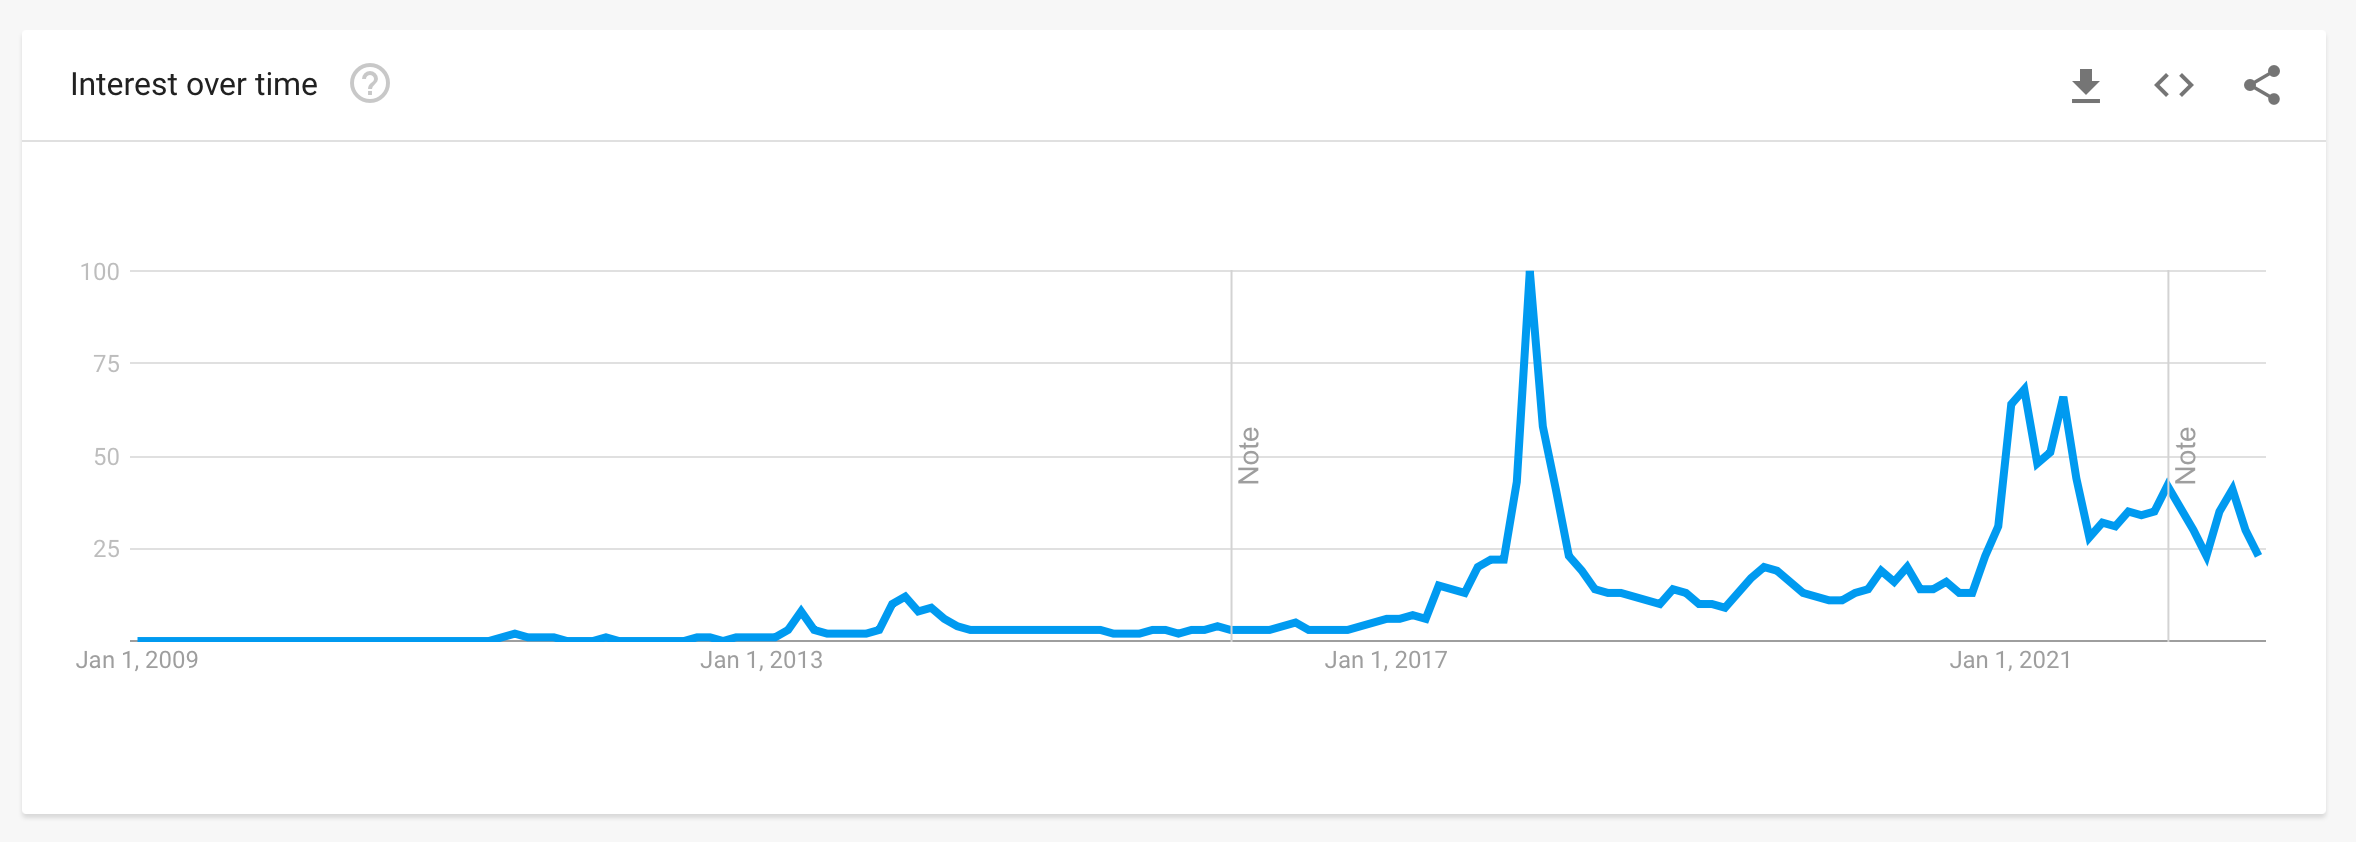
\includegraphics[width=150mm,scale=0.7]{BTC_Popularity.png}
        \caption{Popularity of BTC in Google Searches}
        \label{Figure 3}
    \end{figure}
       \begin{figure}[!htb]
        \centering
        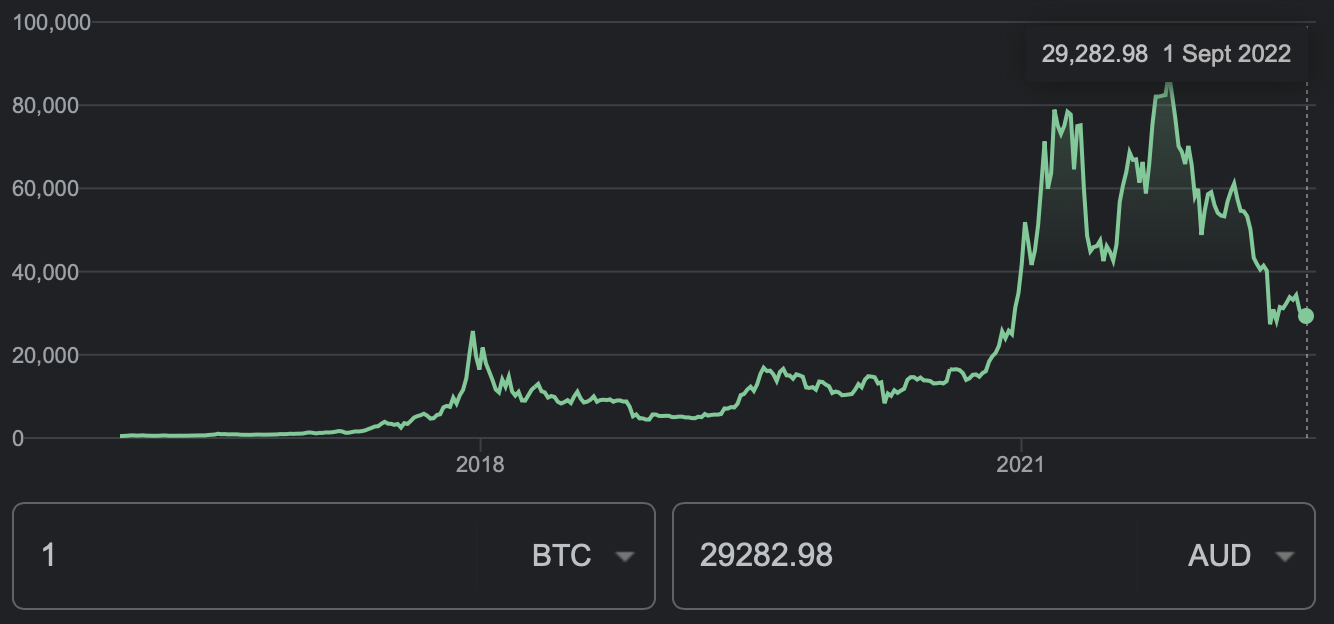
\includegraphics[width=150mm,scale=0.7]{BTC_Price.png}
        \caption{Price trend of BTC}
        \label{Figure 3}
    \end{figure}

\pagebreak

    \subsection{How serious is this problem}

        As mentioned earlier this issue of illegal use of cryptocurrencies is becoming worse and worse every with a sharp increase in the last few years and also a sharp increase expected in the next couple of years at-least due to the increasing popularity of these services. Moreover this is getting worse with the introduction of privacy coins whose sole purpose is to preserve the privacy of users with the downside of a bit higher fees but this makes our point clear that a lot of people are working towards even strengthen privacy in cryptocurrencies with the main motivation being to be able to perform illegal activities on these networks with the lowest chance of getting caught. 

        As we can see in the figure how the relative interest of BTC rose from its early days. There were a very few early investors in BTC which looking at the current prices yielded extremely good results. But as 
        % TBC

\cite{kethineni_cao_2019}

\pagebreak

\section{Related Work}
    
    In this section we will be going through the work that has been previously done in this area of research. As we will go through this section we will realise that a lot of people are already working to break through this issue of governance in cryptocurrencies. As we saw in the last section that illegal and malicious transactions in cryptocurrencies is an ever increasing problem so its very important that some action is taken to add some sort of regulation.


    \subsection{Methods of De anonymization}
        
        Before we dive deep into our own methodology of trying to de anonymize cryptocurrencies it is important we consider and study what methods other people in this field have adopted. In this section we will be going some of those and critically analyze them and use their learnings in our work.
        
        Starting with the most basic ones Narayan Et al\cite{narayanan2016bitcoin} attempted to de anonymize cryptocurrencies to some extent wherein they were aiming to identify what was the nature of the entity on the other end. What they did was simply performed transaction with a huge number of addresses which is definitely not feasible in the current landscape of any cryptocurrencies. This approach fails at a lot of places if we take into account the current situation of cryptocurencies, which includes their prices, their popularity and finally the huge landscape of mixing and shadowing services including privacy coins out there with the sole purpose of preserve privacy of their customers. 
        
        Following this a lot of people worked on automating this process and this was widely accelerated with the advancements in machine learning. Xueshuo Et all\cite{xueshuo2021awap} developed an address classifier to classify addresses based on their network activity. They used public APIs from blockchain.com\cite{blockchain.com} to get data directly from the blockchain. They collected data about transactions and mapped them as vectors in a graph network. After that they developed their model to look out for patterns exhibited by address and were eventually able to classify addresses into various categories like wallets, exchange services, scams, etc with a high success rate. This piece of work shows that it is in deed possible to analyze the blockchain data to group the address and target the malicious ones from there directly vastly bringing down our scope of search when we are only after malicious one. 
        
        Finally we move on to study some advanced methods of de-anonymization. Alex Et al\cite{biryukov2019deanonymization} run a full fledged attack on Bitcoin, Z-Cash and Monero by exploiting the basic principles of a peer to peer network. 
        

\pagebreak

    \subsection{De anonymization of cryptocurrencies}
        
        Muller et al\cite{muller} tried to achieve a similar goal as ours but in a different fashion. The team identified a couple of dark web markets and went on to hunt for the vendors of illegal services. Dark web markets are extremely popular for the sale of illegal drugs, weapons and services and people involved in such activities usually tend to use these services because of the privacy they offer and with the introduction of cryptocurrencies, they have become even more anonymous. They started with public information available on the markets, which is the customer reviews, and from there tried to deduce important information such as time of transaction, value of transaction and the vendor on the market to start with and also took any other information they found. Once they were able to estimate a rough time when the transaction might have occurred they added a buffer of 1 day and looked for a transaction in the blockchain with the same order value. Now the chances that there will be another transaction with the exact value in the specified time frame are negligibly low, so it was relatively easy to mark down the transaction. After they were able to extract the transaction, they took the destination of the money and mapped it to the vendors account.

        In this research they have a done a very good job in identifying the wallet addresses of the vendors, but there are a couple of things we need to critically evaluate as well. Starting with the good, a very good evaluation they did, was they took into account the payment systems of the market and changed their algorithm to identify the vendor accordingly as some markets perform direct transactions whereas some are know to use an escrow service \cite{Fig} for this. A big downside of their research is the the limited expansion. For instance, they are only working with a few dark web markets, and their research purely relies on the customer leaving reviews for the vendor so their approach would be way more effective in markets where customers are encouraged to put reviews and so are vendors to improve their visibility but in markets where this is not the case or reviews are not enforced or even the case where reviewing is not available at all, this approach would either have a very poor performance, or in the last case would completely fail. 

\pagebreak

    \subsection{Anti-Money Laundering in cryptocurrencies}

        With this recent surge in popularity of cryptocurrencies and the related malicious activity governments and financial regulatory authorities all over the world are working on finding ways to track down on this. Governments in some countries have even set up individual authorities and teams with the sole purpose of regulating cryptocurrencies. The most popular way to prevent this in traditional financial institutions is by imposing KYC upon as a regulatory condition. KYC also known as know your customers is a technique which basically all the centralized financial institutions perform to get as much information as possible about their customer before actually letting them inside their institution to safeguard themselves. This way they have all the information about the customer to determine their credit history, their lending power, how good of a customer they would be and finally incase something goes down to track them down. But cryptocurrencies which form the larger part of decentralized finance were made in the first place to avoid this step and because of this any user can open as many accounts / wallets in a currency without essentially providing any information at all.
        
        Hu Et all\cite{hu2019characterizing} developed a machine learning model to identify upcoming clusters of addresses which were extremely likely to be involved in malicious transactions. They started by running the basic bitcoin core client to get transaction data and parsed that into JSON format, and along with that evaluated some ground truth data which was further classified into different categories like malicious users, consumers, etc. After they collected the data they extracted basic features about every transaction such as timestamp, inputs, outputs, with 14 extended features which included but not limited to  linked inputs and output UXTOs (Unspent Transaction Outputs) and used all of this to form a transaction graph. Once they had all this data ready they trained a machine learning model to predict upcoming instances of clusters of malicious addresses.
        % TBC

\pagebreak

    \subsection{Tracking money across cryptocurrency borders}
        In contrast to centralized currencies like dollar, euros, cryptocurrencies, do not have a concept of borders. What that means is that unlike dollar which e.g. is the currency officially used as a legal tender in the United States, and in other countries one has to convert it into the local currency like one would have to convert their dollars into Euros in Europe if they wish to use, cryptocurrencies have no such thing. Its a decentralized form of payment used in the same way worldwide. 

        Yousaf Et al.\cite{tracing_transactions_across_cryptocurrency_ledgers_-_usenix} worked to trace cryptocurrency transaction across multiple currencies. Now this is where they explored beyond the borders of cryptocurrencies. 
        % TBC
        
\pagebreak

    \subsection{Breaking Mixers}
        Now that we are across the concept of mixers and how they work, it is important we go through some of prior work done in order to break through them and be able to trace the transactions that are going through mixers. 
        
        Wang Et all \cite{wang2022zero} worked on solving this very problem to trace the money that was going inside a mixer by first actually determining if a mixer was used in the transaction or not, and if it was they identified some common patterns of people using mixers and mapped the transaction behaviour to the patterns to get to the target address eventually. What they essentially did was pick up a source address and traced the transactions for it until they found a link back to the main address or until they found an indirect link through the value of the transaction. This did involve a very extensive search and traversal of the transactions but they were in the end able to determine if a user used a mixing service or not, and if they did what kind of mixing they perform, i.e. did they just send money to another address and receive it back or did they send money and received it to an entirely different address or even if they sent it and received it back in multiple addresses.
        
        This piece of work does show that it is indeed possible to break through mixers, identify them or find the link between the source and target address in case a mixing service was user. As exhaustive as this would be, it does in the end to some extent cracks through the mixers.
        
\pagebreak

\section{Ethical Considerations}

    Now that we have a good understanding of the problem at our hand and what we are trying to achieve there are a few ethical considerations we need to take into account before we actually start diving into what has been already done and what we will be doing.

    The main point we need to keep in mind here is although we are working with public blockchain data most of the time, we are however trying to get to the real world entity for the associated address, and that is where these ethical concerns kick in. The reason for that is once and if we do reach the real world entity we are dealing with personal data about people which they might not always want everyone to know. This can however can explained in terms of malicious users as the authorities are chasing them up but the work we are doing can potentially be used for non-malicious addresses as well although results may vary.

\pagebreak

\section{Methodology}
 
    Since there is not much information about cryptocurrencies except the information in the public ledger we will need to look outside that scope and see what information we can find about addresses and transactions to make some justified conclusion so as to eventually draw a suspicion explaining how is the address malicious and the conclusions we are making to justify its link with the real world entity. 
    
    The aim over here is now to find a target address either directly or through a transaction and find all the information I can related to it. We have shortlisted a few sources which keep records of information reported by the public, so we will need to scrape through all that information and its related reports to see if we can find something which can identify the person itself. If not we will need to move to the neighbour address and perform a similar search to observe the behaviour of the neighbour address and draw some conclusions. 
    
    The next plan is to identify a few strategic address whose physical location we are aware of with complete certainty and try and find interactions with those addresses. 
    
    \subsection{Step 1 : The target address}
        The first step for us identify the target address. For our research to keep things simple we aimed at an approach which would work for all the addresses rather than specifically illegal activities. This would then enable our work to be used by other researchers in this domain who are interested to see what kind of information we can obtain through this methodology. 
        
        There are 2 ways implemented in our current research to obtain the target address: 
        \begin{enumerate}
            \item The first one, which is primarily used for our development is to pick the latest address in the latest block. 
            For this what we did was used an API 
            In case our starting point is a transaction we will be targeting one of the addresses in the transaction. The information about getting the addresses from the transaction is available readily on the internet through APIs.
        
        Our application can work both on an address or a transaction so our initial call will depend on what we are targeting. 
        
        To extract the address from the transaction we can utilize the public API available from Blockchain.info\cite{blockchain.com}. Blockchain.info is one of the most popular websites which provides the users with multiple services as they require which range from a basic wallet service like any other where users can hold cryptocurrency, trade, buy and sell etc, they have an exchange service which lets the user exchange their cryptocurrency for some other as they like, and they also have specific services for institutions which does not relate to us and finally the one that is of most use to us is the explorer service. The explorer service is basically a platform for users to explore the blockchain online and they have supplemented those with APIs which we are also using for our research. 
        
        \textbf{Information about this source V IMP}
        
        \textbf{Url : GET} \url{https://blockchain.info/rawtx/{{tx_hash_or_id}}}
        Every transaction in the blockchain gets a hash value when generated and verified so this API takes in that as a path variable and returns the response below for a sample random transaction we picked up. The data model for the response is also shown in figure \cite{Fig}.
        
        \textbf{Sample Response: }
        \lstinputlisting[caption=A single transaction from the blockchain]{SingleTx.json}
        
        As we can see from the sample response we can directly access the input and output address as our target and move on to the next step which is getting data about the individual address itself.
        
        Now the task for us is to pick up the address in question and identify as much information as possible about it before we move on.
        
            \item As an extension to the current functionality we have also given the user the option to input an address so that he can look for the information he is after rather than just picking up the latest address which is not always what one is after. 
        
        \end{enumerate}
        
        After we have obtained the address we pass it onto our next service which is responsible for extracting the data related to the address, then followed by data processing to turn the raw data into meaningful from which we can actually make some sort of conclusions. This next step is divded into multiple ones because of the complexity and tasks involved starting from getting basic data from the blocjchain, followed by more complex web scraping and natural language processing to make some reasonably justified conclusions.
        
        
    \subsection{Step 2 : Metadata about the address}
    
        \textbf{Collection of metadata about the address or transaction}. 
        This is the tricky part for us since our research purely relies on data publicly available which can be on the blockchain or information reported by private entities on the Internet. This information is very limited specially if we pick up a random address for our investigation and the reason for this is due to the pseudo-anonymous nature of cryptocurrencies. In cryptocurrencies a person can essentially set up as many addresses or so called account numbers as he wishes without any personally identifiable information in contrast to traditional banking system where a proper KYC is mandatory before one can use those services. Due to this the only information readily available is the public key of the user using the services which is his wallet address. What we can do is use that wallet address to query different sources to get as much information as possible about it. For this we be utilizing a mix of API services and also build a web scraping service to extract information no available from API due to reasons highlighted below.
        
        
        
        Firstly we will be utilizing an API from Blockchain.info\cite{blockchain.com} to get basic information about the address. The API below from this source gives us
        \textbf{Url : GET} \url{https://blockchain.info/rawaddr/{{address_id}}}
        
        This API takes in the wallet address which is the publicly available on the blockchain as a path variable and gives all the information about it directly from the blockchain. The data structure of the response is shown in the figure\cite{} from which we will observe the interactions of the address inside the blockchain.
        
        \textbf{Sample Response: }
        
        \lstinputlisting[caption=A single address from the blockchain]{SingleAddr.json}
        
        The main information we need to extract from here is the interactions of the address throughout the blockchain. As we can see from the sample response we get a list of transactions in the \textbf{txs} object though which we can loop through to get to the immediate neighbours of the address. We refer immediate neighbours to addresses which directly interact with the address though a transaction where our target address can either be the sender or the receiver. 
        
\pagebreak 

    \subsection{Step 3 : Web Scraping}
        Now that we have most of the metadata about the address we need to understand the nature of the address, we will starting digging into the address to find links to the real world. For this we will be building a web scraping service to go through a couple of identified online sources which seem have data which can help us get as close to the real world entity as possible. 
        
        When it comes to web scraping we will be downloading the entire page as an HTML instead of using APIs and then parsing the page element by element. This approach has both advantages and dis-advantages but in our cases the advantages outweigh the negatives so we are using this approach. Firstly when it comes to APIs, these sources are not best known to provide these services so getting an API key is very hard. We applied for an API key but its been over months since we have got anything so we decided to use the web crawling service as it will also give us more control over what data we can process. And finally APIs always have this security throttling feature against Denial of Service attacks so we can bypass this while scraping the web as we are acting as if a lot of users are accessing the web page which is a very normal behaviour and most websites do not have any restriction to the number of users who can access their page.
        
        For the web scraping of the page obtained from the sources we have to tailor write our code to adapt to the HTML returned from the page to target and extract data from the exact section of the page we are after. The main section of the page we are interested is the scam alerts \cite{}. In order to do so we are using the python's\cite{python.org} beautiful soup\cite{beautiful_soup_documentation} library which is well known to be used for these applications where we want to read exact sections from an HTML page.
        
        % Insert Code for the scraping
        
        The sources we are targeting right now are 
        \begin{enumerate}
            \item Bitcoin Who is Who\cite{bitcoinwhoswho}
            \item Hash XP\cite{hashxp.org}
        \end{enumerate}
        In the sections below we will go though in detail the data provided by each source in detail but breifly these 2 sources provide nearly the same information except in some case one is known to have more information about the address than the other so it is always good to have 2 sources and also helps in better data validation. In the end we cannot completely rely on this information as this is publicly sourced and there are high chances of false positives as well so we have to take a cautious approach when analyzing this data and making further conclusions. 
        
        In short these sources provide some very good insights about an address such as the basic information from the blockchain such as balance(s), transaction(s), but the main data we are interested in from these sources is the scam alert which we will be scraping using our service. These are reports submitted by people from all over the world wherein an address was known to perform a malicious activity. We will analyzing that data to make further conclusions about the address.
        
        In the web scraping service what we are doing is starting to get data about the actual address itself and then moving on to the neighbours of the address identified earlier through it transactions and getting data about them to observe and understand the behaviour of the address though the neighbours and if needed might move the second neighbours as well which is the addresses to which the direct neighbours have interacted with.
        \begin{itemize}
            \item BitcoinWhoIsWho : From this source when we download the page we get HTML of the sample page attached in fig \cite{} . From here the main data we are after is the scam alerts section which in this case a bunch of reports sent through by random people online who have either witnessed or been targeted by a particular address. 
            % \item HashXp : 
        \end{itemize}
        
        After we have extracted the data from the 2 sources we are saving it in a seperate file to analyze and understand what sort of information we can get and what conclusions we can make about the target address from the data about the address and its neighbours.

\pagebreak

    \subsection{Step 4 : Analyzing data obtained to get some results}
    
        Once we have got all the data from the sources above we dump everything into a single file to try and visualise the relationships between the target addresses and its neighbours with the vital information to make some justified reasonable conclusions. \textbf{We need to keep in mind our goal in the end is to get close to the real world entity associated with the address, not identify whether its legal or illegal as that work has already been done.} 
        
\pagebreak

    \subsection{Step 5 : Validation of Results}
    
    
        
\pagebreak

\section{Experiment Performed}      
    In this section we will be going through how and by what means we performed the above mentioned methodology. We will explain how we derived the data and then how we used it in our application and eventually how we came up with the results presented in the following section.
    
    \subsection{Selection of Data Set}
        For the data to be used in the experiment to check if our approach yields any results or not we rounded our radius down to 2 data sets
        \begin{itemize}
            \item Elliptic Data Set\cite{elliptic} \cite{weber2019anti}
            \item BitcoinHeistRansomwareAddressDataset\cite{akcora2019bitcoinheist}
            \item Twitter Data
            \item BTCAbuse Report Data
        \end{itemize}
        
        Both data sets have enough information for us to be able to perform our simulation to get data about the address and its neighbours. The elliptic data set has an advantage because of the number of features it maintains for each and every address but then again we are not performing any machine learning analysis at this point that those features would be of use for us. Also, after some manual experimentation we found that that elliptic data set does not have real data rather the addresses were masked so that made the data set essentially impossible for us to use since we are looking for real world on information about the addresses on the internet. So, to conclude we decided to use the BitcoinHeistRansomwareAddressDataset since it contains real world information and is also very extensive in terms of data which we will go in detail in the next section.
        
\pagebreak
    
    \begin{center}
        \begin{tabular}{||c c||} 
             \hline
             \textbf{Scam Label} & \textbf{Count}  \\ [0.5ex] 
             \hline\hline
             princetonCerber & 9223  \\ 
             \hline
             princetonLocky & 6625  \\
             \hline
             montrealCryptoLocker  & 9315  \\
             \hline
             montrealCryptXXX & 2419  \\
             \hline
             paduaCryptoWall & 12390  \\ [1ex] 
             \hline
              montrealWannaCry & 28  \\ [1ex] 
             \hline
              montrealDMALockerv3 & 354  \\ [1ex] 
             \hline
              montrealCryptoTorLocker2015 & 55  \\ [1ex] 
             \hline
              montrealSamSam & 62  \\ [1ex] 
             \hline
              montrealNoobCrypt & 483  \\ [1ex] 
             \hline 
             montrealDMALocker  & 251  \\ [1ex] 
             \hline
              montrealGlobe & 32  \\ [1ex] 
             \hline
              montrealEDA2 & 6  \\ [1ex] 
             \hline
               paduaKeRanger & 10  \\ [1ex] 
             \hline
               montrealVenusLocker & 7  \\ [1ex] 
             \hline
               montrealXTPLocker & 8  \\ [1ex] 
             \hline
               paduaJigsaw & 2  \\ [1ex] 
             \hline
               montrealGlobev3 & 34  \\ [1ex] 
             \hline
               montrealJigSaw & 4  \\ [1ex] 
             \hline
               montrealXLockerv5.0 & 7  \\ [1ex] 
             \hline
               montrealXLocker & 1  \\ [1ex] 
             \hline
               montrealRazy & 13  \\ [1ex] 
             \hline
               montrealCryptConsole  & 7  \\ [1ex] 
             \hline
               montrealGlobeImposter & 55  \\ [1ex] 
             \hline
               montrealSam & 1  \\ [1ex] 
             \hline
               montrealComradeCircle & 1  \\ [1ex] 
             \hline
              montrealAPT & 11  \\ [1ex] 
             \hline
              white & 2875284  \\ [1ex] 
             \hline
        \end{tabular}
    \end{center}
    
       \begin{figure}
            \centering
            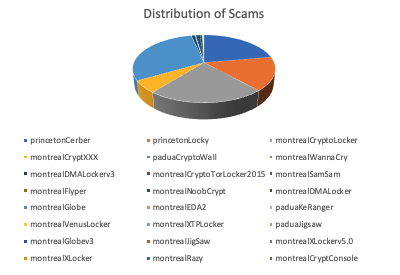
\includegraphics[width=150mm,scale=0.7]{Distribution of Scams.png}
            \caption{Distribution of scams in the data }
            \label{Figure 3}
        \end{figure}

\pagebreak
    \subsection{The Data Set}
        
        Now that we have decided to use the BitcoinHeistRansomwareAddressDataset we will explain in detail what kind of data we are getting from the data and how we used in the experiment itself.
        
        To start with the data set is a collection of 2916697 addresses, out of which 41413 have been labelled to being involved in one or other identified scam, with the following headers and the ones of our interest specifically have been explained.
        \begin{enumerate}
            \item address : The address about which the row contains information.
            \item year
            \item day
            \item length 
            \item weight : Weight defines the merge behavior, the ratio of input to output addresses.
            \item count 
            \item looped
            \item neighbours : The number of recorded neighbours of the address.
            \item income : This is the income of the address in Satoshi amount (1 bitcoin = 100 million satoshis).
            \item label : This is label associated with each address to identify what is the nature of the address. The distribution of labels can be found in fig \ref{Figure 3} and 'White' refers to a clean address as determined by the authors of the data set.
        \end{enumerate}
        
        From this entire data set, we are primarily interested in the malicious ones which are 41413 out of the total roughly 3 million addresses. This however does show that this is a very unevenly distributed data set. But for the sake of our experiment we will only deal with the malicious ones as our primary goal is to extract data about addresses involved in these kinds of transactions. The dataset also has the identified neighbours of every address, identified at time of data collection which will help us prioritize the addresses over others as addresses with more neighbours are more likely to give us better results than others.

\pagebreak

    \subsection{Processing the data set}
        Now since we need to explore the data as well as access it in our python script, the most efficient way of doing this was to import it into an SQL database as conventional csv readers such as Microsoft Excel cannot handle such large data sets. 
        
        After the data set was imported into the SQL database we could make direct queries on the DB both in our python script and also directly through the MySQL interface. After this we access the data in our python script and we specifically target the malicious addresses and apply our algorithm described in fig \ref{Figure 3} to get the data and process to get the results highlighted in the next section.
        
    
\pagebreak


\section{Problems Encountered}
    
    Every research is a problem unsolved and so we also faced a few issues in our work. In this section we will be going through the problems we faced while performing this research and what solutions we came up to overcome them. 
    
    \subsection{Very Limited Data} 
    
        This is the essence of the problem we are trying to solve. Directly the blockchain provides us with all the information stored in the ledger which is basic financial information such as money held, transactions made 
        
    \subsection{Lack of reliable APIs}
    
        All the sources we used above to collect our data have APIs available but were not accessible to us and also had rate limits which would hinder our work. Most of the services had free APIs available and we used them wherever feasible considering the rate limit. For instance we used blockchain.info's free API to collect neighbours of an address as we didn't need to make thousands of calls over there considering the rate limit was maximum 10 calls per minute so we were able to get all the required data within a span of a couple of hours. For the rest of the data which we scraped online from BitcoinWhoIsWho, we could not use the APIs. The reasons for that being, first, we applied for an API key in the early days however failed to receive any response from the party responsible for issuing an API key and also we needed to access that page more than tens of thousands of times so no API would have such a generous limit for us to be able to do that. So, to overcome this we built the web scraping application which just imitates a user on the website and the website would just consider it as a lot of people visiting it rather than through an API where they could consider a Denial of Service Attack and block us.
        
    \subsection{IP getting blocked from One of the APIs}
        % Blockchain.info blocking my home IP
        We were constantly accessing Blockchain.info API to get neighbour addresses of the target. We were trying to hit the API nearly 100 times plus a second and tried over a number of days. After digging a bit deeper we found that the API has a rate limit of 10 calls maximum per minute so we adapted our program to do that but turns out doing that also too many times blocks our IP. So in the last few weeks we had one of our IPs blocked due to making too many requests and every time we tried accessing it through the IP, we got a HTTP-Status 429\cite{Error_429} which is an error status for making too many calls. So, for this we had to switch networks and adapted our approach to collect all the data in one go and then process it locally as required. 
            
    \subsection{Very Slow Results Data Collection}  
        The Python script we developed initially was a completely synchronous program which meant one step ran after another one has finished. This was working fine for test data-sets where we were just checking if our program works or not with a couple of address but when we actually started performing our experiment with thousands of addresses our program throttled exponentially. There were multiple reasons for this and overall this resulted into such a slow program that it was estimated that our experiment would take over a month to just execute and then we had to analyze the results after that which was definitely not feasible considering the time frame we had. So, to overcome this we refactored the entire script to be asynchronous and concurrently perform multiple tasks. For this we used the Python's AsyncIo\cite{asyncio} library which basically collects all the methods/tasks to be run together and runs them in parallel using co-routines. This way were we were able to analyze hundreds of addresses at once and also their neighbours which meant that at one point we were processing thousands of addresses and that too didn't take more than a few minutes for every execution. 
        % Maybe the 10K at once issue
    
\pagebreak

\section{Critical Judgement and Evaluation of Results}

\pagebreak

\section{Future Work}

\pagebreak

\section{Conclusion}

\pagebreak

\section{Abbreviations}
\pagebreak

% Appendix with code and stuff
\pagebreak
\bibliographystyle{ieeetr}
\bibliography{citation} 
\end{document}